\chapter{Verifica e validazione}
\label{cap:verifica-validazione}

\par In questa sezione sono riportati i test effettuati durante lo svolgimento del progetto. La fase di testing è stata suddivisa in due sottofasi: verifica e validazione (V\&V). La verifica consiste nell’accertare che il software sia conforme alle specifiche, e può essere condotta senza eseguire il codice. Le attività di analisi statica includono la revisione e l’ispezione dei processi, dei \gls{requisiti}, del design e del codice sorgente. Quest’ultima può avvenire tramite una lettura approfondita del codice o mediante una revisione sistematica e mirata. La validazione, invece, riguarda l’analisi dinamica del software, finalizzata ad accertare il soddisfacimento dei \gls{requisiti} e delle aspettative dal punto di vista dell’utente finale. Le attività di validazione comprendono sia test automatici che manuali.

\lstdefinelanguage{JavaScript}{
  keywords={break, case, catch, continue, debugger, default, delete, do, else, finally, for, function, if, in, instanceof, new, return, switch, this, throw, try, typeof, var, void, while, with, let, const},
  keywordstyle=\color{blue}\bfseries,
  ndkeywords={class, export, boolean, throw, implements, import, this},
  ndkeywordstyle=\color{darkgray}\bfseries,
  identifierstyle=\color{black},
  sensitive=false,
  comment=[l]{//},
  morecomment=[s]{/*}{*/},
  commentstyle=\color{gray}\ttfamily,
  stringstyle=\color{red}\ttfamily,
  morestring=[b]',
  morestring=[b]"
}

\section{Test automatici}

\par Il testing automatizzato è una tecnica che prevede la configurazione di un ambiente di test e la progettazione di una o più suite che vengono eseguite automaticamente, confrontando i risultati effettivi con quelli attesi. Ogni test dovrebbe essere veloce, indipendente, affidabile e riutilizzabile. I test automatici non sostituiscono i test manuali né eliminano la necessità di una revisione “umana”; tuttavia, forniscono una misura oggettiva della qualità del software e contribuiscono a ottimizzare il ciclo di sviluppo, individuando rapidamente errori che potrebbero sfuggire all’osservazione manuale, specialmente in contesti di \gls{continuous integration}.

\vspace{10pt}
\par\noindent La progettazione, scrittura e manutenzione dei test automatici hanno richiesto uno sforzo considerevole; tuttavia, data la ridotta finestra temporale dello stage, l’automatizzazione si è rivelata essenziale nel lungo periodo. Essa ha infatti fornito un riscontro continuo sulla qualità del software durante lo sviluppo, riducendo il carico di lavoro legato all’esecuzione dei test manuali. Inoltre, ha consentito di raggiungere una copertura del codice del 100\% (come attestato dal report di Codecov in figura \ref{fig:report_codecov}), un risultato difficilmente ottenibile con il solo testing manuale.

\begin{figure}[H]
  \centering 
  \fbox{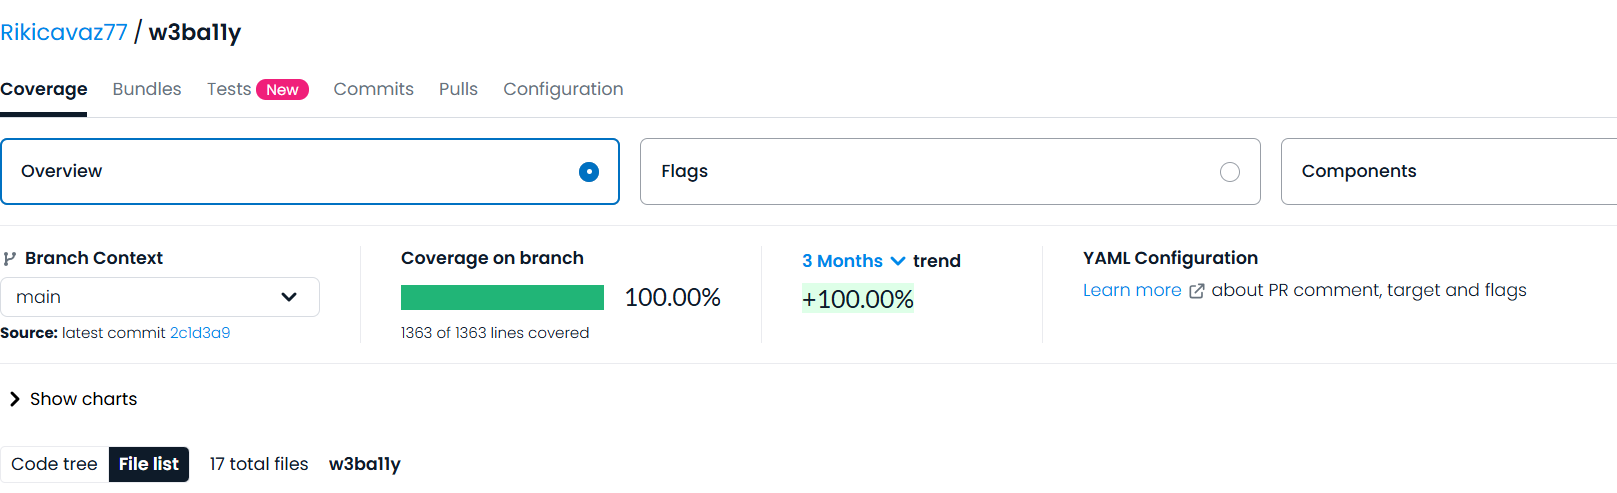
\includegraphics[width=0.9\columnwidth]{test/coverage.png}}
  \caption{Copertura del codice - report di Codecov}
  \label{fig:report_codecov}
\end{figure}

\par\noindent I test automatici vengono eseguiti a ogni apertura, aggiornamento o chiusura di una \gls{pull request}, garantendo che tutto il codice rilasciato superi i test e mantenga una copertura uniforme. Dal punto di vista architetturale e organizzativo, i test rispecchiano fedelmente la struttura del \textit{core} dell’estensione, risultando più leggibili e manutenibili. 

\vspace{10pt}
\begin{samepage}
  \dirtree{%
    .1 tests.
    .2 controller.
    .2 model.
    .2 services.
    .3 strategy.
    .2 utils.
    .2 view.
  }
\end{samepage}

\vspace{10pt}
\par\noindent Per mantenere l’isolamento tra l'estensione e l’ambiente di test, ciascun file testato deve terminare con la seguente porzione di codice:

\vspace{10pt}
\begin{samepage}
\begin{lstlisting}[language=JavaScript]
  /* istanbul ignore next */
  if (typeof module !== 'undefined' && typeof module.exports !== 'undefined') {
    module.exports = KeywordHighlighter;
  }
\end{lstlisting}
\end{samepage}

\vspace{10pt}
\par\noindent Questo approccio consente di importare i moduli all’interno dei file di test tramite la seguente istruzione:

\vspace{10pt}
\begin{samepage}
\begin{lstlisting}[language=JavaScript]
  const KeywordHighlighter = require('@keyword/services/keyword_highlighter');
\end{lstlisting}
\end{samepage}

\vspace{10pt}
\par\noindent La tabella \ref{tab:test-automatici} riporta i test di unità e di integrazione eseguiti.

\renewcommand{\arraystretch}{1.5}
\begin{longtable}{>{\raggedright\arraybackslash}p{0.65\textwidth} >{\raggedright\arraybackslash}p{0.25\textwidth}}
\caption{Tabella dei test automatici}
\label{tab:test-automatici} \\
\hline\hline
\textbf{Suite di test} & \textbf{\% di superamento dei test}\\
\endfirsthead
    
\caption[]{Tabella dei test automatici (continua)} \\
\hline\hline
\textbf{Suite di test} & \textbf{\% di superamento dei test} \\ 
\endhead
    
\multicolumn{2}{r}{{Continua nella prossima pagina}} \\ 
\endfoot
    
\hline
\endlastfoot

\hline
\textbf{Keyword} \textit{(keyword.test.js)}: verifica il corretto funzionamento del modello relativo alle parole chiave. & 100\% \\
\hline
\textbf{AnalysisResultView} \textit{(analysis\_result\_view.test.js)}: verifica il corretto funzionamento del componente responsabile della visualizzazione dei risultati relativi all’analisi di una parola chiave. & 100\% \\
\hline 
\textbf{KeywordListView} \textit{(keyword\_list\_view.test.js)}: verifica il corretto funzionamento del componente responsabile della visualizzazione delle liste di parole chiave per ciascuna tipologia. & 100\% \\
\hline 
\textbf{KeywordView} \textit{(view.test.js)}: verifica il corretto funzionamento della view principale, responsabile della gestione della \textit{dashboard} e delle sottoview. & 100\% \\
\hline 
\textbf{KeywordController} \textit{(controller.test.js)}: verifica il corretto funzionamento delle operazioni di gestione delle parole chiave (funzionalità non dipendenti dal \gls{dom} e non sufficientemente specifiche da giustificare una suite dedicata). & 100\% \\
\hline 
\textbf{KeywordController - DOM} \textit{(controller\_dom.test.js)}: verifica il corretto funzionamento delle operazioni del controller che richiedono l’interazione con il \gls{dom}. & 100\% \\
\hline 
\textbf{KeywordController - sorting} \textit{(controller\_sorting.test.js)}: verifica la funzionalità di ordinamento delle parole chiave. & 100\% \\
\hline
\textbf{KeywordController - filtering} \textit{(controller\_filtering.test.js)}: verifica la funzionalità di filtraggio delle parole chiave. & 100\% \\
\hline
\textbf{KeywordController - pagination} \textit{(controller\_pagination.test.js)}: verifica la logica di gestione della paginazione delle parole chiave. & 100\% \\
\hline
\textbf{KeywordController - highlight} \textit{(controller\_highlight.test.js)}: verifica la logica di gestione dell’evidenziazione delle parole chiave. & 100\% \\
\hline
\textbf{KeywordController - events} \textit{(controller\_events.test.js)}: verifica il corretto funzionamento dell’associazione (binding) degli eventi. & 100\% \\
\hline
\textbf{KeywordController - init} \textit{(controller\_init.test.js)}: verifica le funzionalità di inizializzazione e di aggiornamento del controller, nonché l’integrazione tra i componenti dell’architettura. & 100\% \\
\hline
\textbf{TreeWalkerManager} \textit{(tree\_walker\_manager.test.js)}: verifica la corretta gestione dell’oggetto \textit{TreeWalker}. & 100\% \\
\hline
\textbf{TextProcessor} \textit{(text\_processor.test.js)}: verifica il corretto comportamento delle funzioni di utilità legate all’analisi e all’elaborazione testuale. & 100\% \\
\hline
\textbf{TagAccessor} \textit{(tag\_accessor.test.js)}: verifica il corretto comportamento delle funzioni di utilità dedicate all’accesso e alla lettura del contenuto dei tag \gls{html}. & 100\% \\
\hline
\textbf{WordCounter} \textit{(word\_counter.test.js)}: verifica le funzionalità di conteggio delle parole e di estrazione di quelle più frequenti. & 100\% \\
\hline
\textbf{KeywordHighlighter} \textit{(keyword\_highlighter.test.js)}: verifica la funzionalità di evidenziazione delle parole chiave all’interno della pagina. & 100\% \\
\hline
\textbf{KeywordAnalyzer} \textit{(keyword\_analyzer.test.js)}: verifica la funzionalità di analisi delle parole chiave. & 100\% \\
\hline
\textbf{KeywordAnalysisStrategy} \textit{(keyword\_analysis\_strategy.test.js)}: verifica il corretto comportamento della struttura astratta, assicurandosi che l’istanziazione diretta sia impedita e che i metodi non implementati generino un errore. & 100\% \\
\hline
\textbf{StagedAnalysisStrategy} \textit{(staged\_analysis\_strategy.test.js)}: verifica il corretto funzionamento dell’implementazione concreta della \textit{strategy}, basata su un’analisi “per fasi” (staged). & 100\% \\
\hline
\textbf{AllInOneAnalysisStrategy} \textit{(all\_in\_one\_analysis\_strategy.test.js)}: verifica il corretto funzionamento dell’implementazione concreta della \textit{strategy}, basata su un’analisi compatta e unificata. & 100\% \\
\hline
\textbf{Utils} \textit{(utils.test.js)}: verifica il corretto comportamento delle funzioni di utilità. & 100\% \\
\end{longtable}

\section{Test manuali}

\par L’estensione è stata testata su un insieme di pagine web differenti per dimensione (in termini di profondità del \gls{dom}) e lingua (inglese o italiana), con l’obiettivo di verificarne il corretto funzionamento mediante osservazione manuale. La tabella \ref{tab:test-manuali} riporta i test manuali eseguiti.

\renewcommand{\arraystretch}{1.5}
\begin{tabularx}{\textwidth}{>{\raggedright\arraybackslash}X >{\raggedright\arraybackslash}X}
\caption{Tabella dei test manuali}
\label{tab:test-manuali} \\
\hline\hline
\textbf{Sito web} & \textbf{Esito dei test}\\
\endfirsthead
    
\caption[]{Tabella dei test manuali (continua)} \\
\hline\hline
\textbf{Sito web} & \textbf{Esito dei test} \\ 
\endhead
    
\multicolumn{2}{r}{{Continua nella prossima pagina}} \\ 
\endfoot
    
\hline
\endlastfoot

\hline
\textbf{W3Schools} - JavaScript Tutorial (\url{https://www.w3schools.com/js/}) & Tutti i test manuali sono stati superati con successo, inclusa l'analisi di parole chiave “spezzate” su più tag \gls{html} (es. “JavaScript Tutorial”). L’unica eccezione riscontrata nelle prime fasi di sviluppo riguardava il mancato rilevamento dei meta tag keywords e description. Il problema era dovuto al fatto che, contrariamente alle convenzioni più comuni, il valore dell’attributo \textit{name} iniziava con una lettera maiuscola. La soluzione adottata è stata l’aggiunta del flag di confronto “case-insensitive” nel selettore. \\
\hline
\textbf{W3Schools} - JavaScript Regular Expressions (\url{https://www.w3schools.com/js/js\_regexp.asp}) & Tutti i test manuali sono stati superati con successo. \\
\hline
\textbf{Corriere della Sera} - HomePage (\url{https://www.corriere.it/}) & Tutti i test manuali sono stati superati con successo, sebbene con prestazioni non sempre ottimali, a causa della complessità del sito in questione. \\
\hline
Siti web partecipanti al concorso \textbf{Accattivante Accessibile}, organizzato dall’Università degli Studi di Padova (\url{https://web.math.unipd.it/CAA/classifica.html}) & Tutti i test manuali sono stati superati con successo. Durante l’analisi del sito \textit{BookOverflow}, è emerso un caso particolare non gestito: una singola parola “spezzata” su più tag \gls{html} (es. “BookOverflow”). Questa situazione è stata valutata come un’eccezione poco significativa, non tale da giustificare una gestione più granulare, che avrebbe inciso negativamente sulle prestazioni. \\
\hline
\textbf{Nasce, Cresce, Ignora} - The Killer, la recensione (\url{https://nascecresceignora.it/the-killer-la-recensione-un-thriller-freddo-e-glaciale/}) & Tutti i test manuali sono stati superati con successo, inclusa l'analisi di parole chiave “spezzate” su più tag \gls{html} (es. “David Fincher”) e l’estrazione delle keyphrase più frequenti (es. “The Killer”). \\
\hline
\textbf{Nasce, Cresce, Ignora} - Pixar: I migliori film (\url{https://nascecresceignora.it/pixar-i-migliori-film-secondo-letterboxd/}) & Tutti i test manuali sono stati superati con successo. \\
\hline
\textbf{Nasce, Cresce, Ignora} - Death Stranding 2: On The Beach (\url{https://nascecresceignora.it/death-stranding-2-on-the-beach-pubblicato-nuovo-trailer-gameplay/}) & Tutti i test manuali sono stati superati con successo. \\
\hline
\textbf{Nasce, Cresce, Ignora} - The Last of Us in concerto (\url{https://nascecresceignora.it/the-last-of-us-in-concerto-gustavo-santaolalla-annuncia-2-date-italia/}) & Tutti i test manuali sono stati superati con successo. \\
\hline
\textbf{la Repubblica} - HomePage (\url{https://www.repubblica.it/}) & Tutti i test manuali sono stati superati con successo. \\
\hline
\textbf{TradingView} - HomePage (\url{https://it.tradingview.com/}) & Tutti i test manuali sono stati superati con successo, sebbene con prestazioni non sempre ottimali, a causa della complessità del sito in questione. \\
\hline
\textbf{GitHub} - HomePage (\url{https://github.com/}) & Tutti i test manuali sono stati superati con successo. \\
\hline
\textbf{STEM Unipd} - HomePage (\url{https://stem.elearning.unipd.it/}) & Tutti i test manuali sono stati superati con successo. Data la presenza di numerosi tag nascosti, la maggior parte delle parole chiave più frequenti non risulta direttamente visibile all’utente. Per rendere più chiara questa situazione, è stato inserito un messaggio esplicativo nella sezione principale dell’estensione. \\
\hline
\textbf{Computer Science Unipd} - HomePage (\url{https://informatica.math.unipd.it/}) & Tutti i test manuali sono stati superati con successo. \\
\hline
\textbf{THINKY} - HomePage (\url{https://prodotto.netlify.app/}) & Tutti i test manuali sono stati superati con successo. Cambiando il tema del sito da chiaro a scuro, il rapporto di contrasto dei colori all’interno dell’estensione risultava compromesso. Il problema è stato risolto forzando lo schema di colori da utilizzare. \\
\hline
\textbf{Vite} - HomePage (\url{https://vite.dev/}) & Tutti i test manuali sono stati superati con successo. Durante l’evidenziazione delle parole chiave contenute nel tag H1, il testo risultava nascosto, lasciando un riquadro vuoto. Il problema è stato risolto azzerando gli stili preimpostati del tag genitore. \\
\end{tabularx}

\newpage

\subsection{Questionario SUS}

\par Il questionario \gls{sus} è stato compilato da 12 utenti, tutti appartenenti all’Università degli Studi di Padova e quindi familiari con il contesto d’uso principale dell’estensione, rivolta principalmente a sviluppatori web. Il template standard è composto da 10 affermazioni (item), bilanciate tra positive e negative, a cui il rispondente assegna un punteggio da 1 a 5 in base al proprio grado di accordo o disaccordo, secondo un intervallo che va da “Fortemente in disaccordo” a “Fortemente d’accordo”. Questo metodo di valutazione prende il nome di \textit{scala Likert} ed è utilizzato per ottenere una valutazione affidabile dell’usabilità di un sistema senza un dispendio eccessivo di risorse.

\vspace{10pt}
\par\noindent Il calcolo del punteggio complessivo segue i seguenti criteri:
\begin{itemize}
  \item Sottrarre 1 dal punteggio per ciascuna domanda dispari;
  \item Sottrarre il punteggio da 5 per ciascuna domanda pari;
  \item Sommare i risultati ottenuti e moltiplicare il totale per 2,5. 
\end{itemize}

\vspace{5pt}
\par\noindent Il punteggio medio ottenuto è pari a \textbf{79}, superiore alla media di riferimento di 68, generalmente considerata indicativa di una buona usabilità. Di seguito sono riportati i grafici relativi alle risposte fornite per ciascuna delle 10 domande del questionario.

\subsubsection*{Domanda 1}

\vspace{5pt}
\begin{minipage}{\textwidth}
  \par\noindent La figura \ref{fig:sus_q1} mostra le risposte alla prima domanda del questionario \gls{sus}.
  \begin{figure}[H]
    \centering
    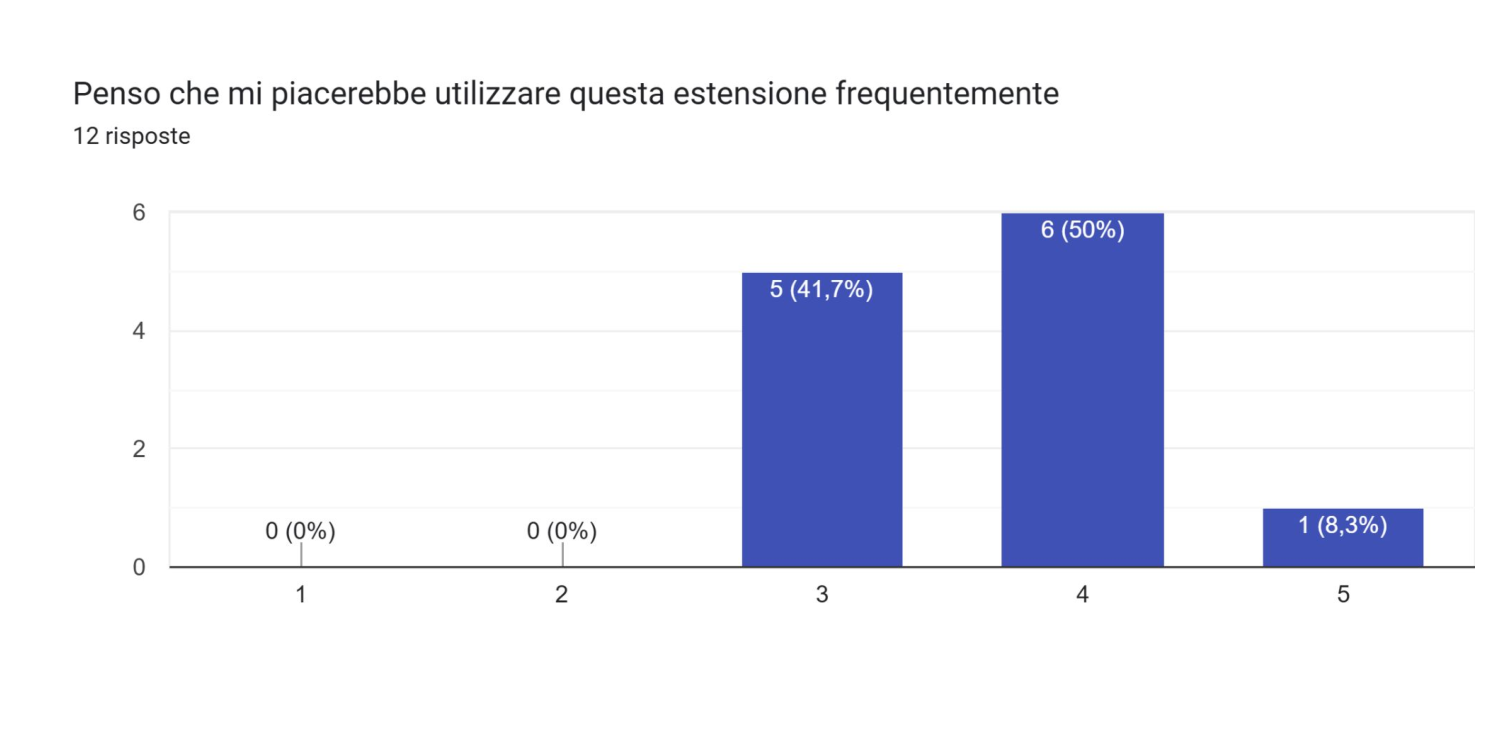
\includegraphics[width=0.95\columnwidth]{sus/domanda_1.pdf}
    \caption{Risposte alla domanda 1}
    \label{fig:sus_q1}
  \end{figure}
\end{minipage}

\subsubsection*{Domanda 2}

\vspace{5pt}
\begin{minipage}{\textwidth}
  \par\noindent La figura \ref{fig:sus_q2} mostra le risposte alla seconda domanda del questionario \gls{sus}.
  \begin{figure}[H]
    \centering
    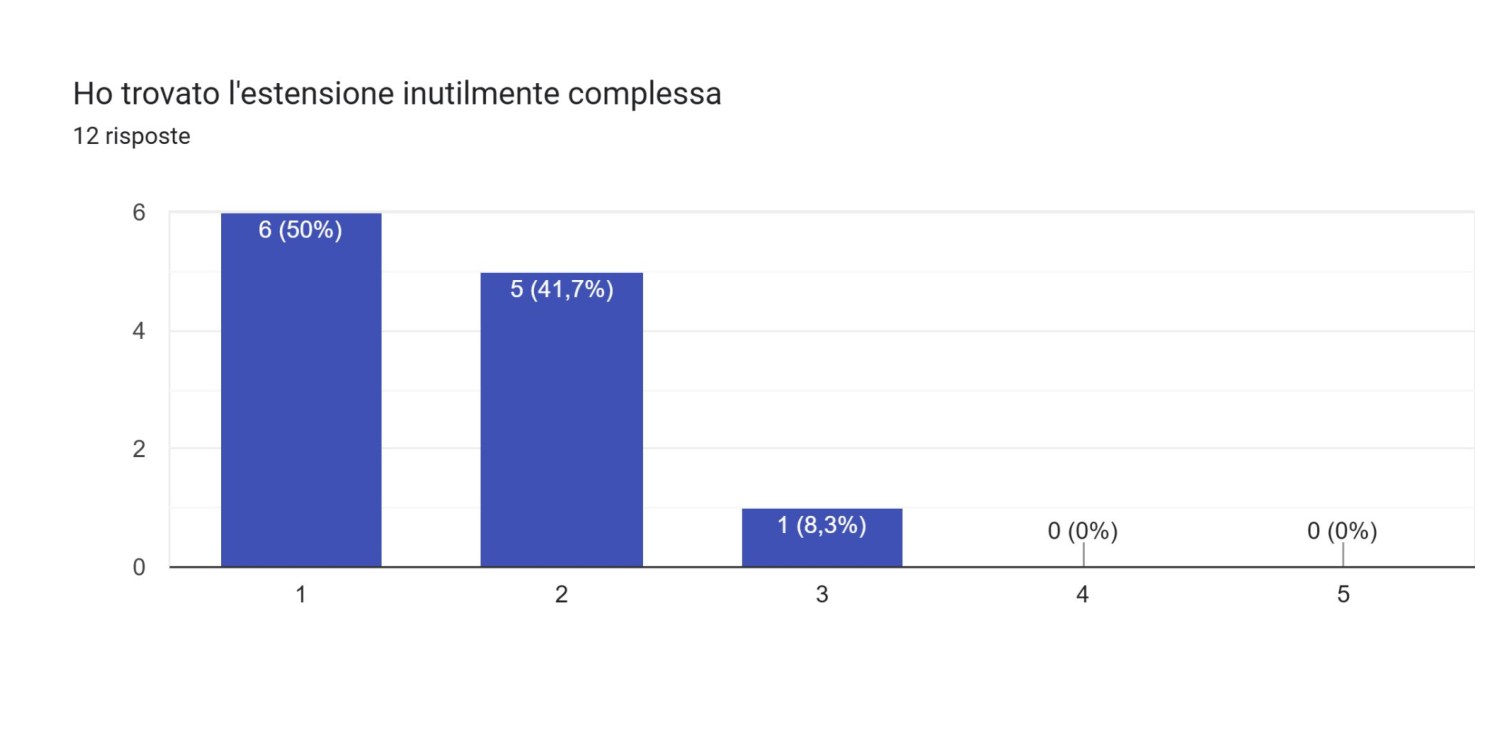
\includegraphics[width=0.95\columnwidth]{sus/domanda_2.pdf}
    \caption{Risposte alla domanda 2}
    \label{fig:sus_q2}
  \end{figure}
\end{minipage}

\subsubsection*{Domanda 3}

\vspace{5pt}
\begin{minipage}{\textwidth}
  \par\noindent La figura \ref{fig:sus_q3} mostra le risposte alla terza domanda del questionario \gls{sus}.
  \begin{figure}[H]
    \centering
    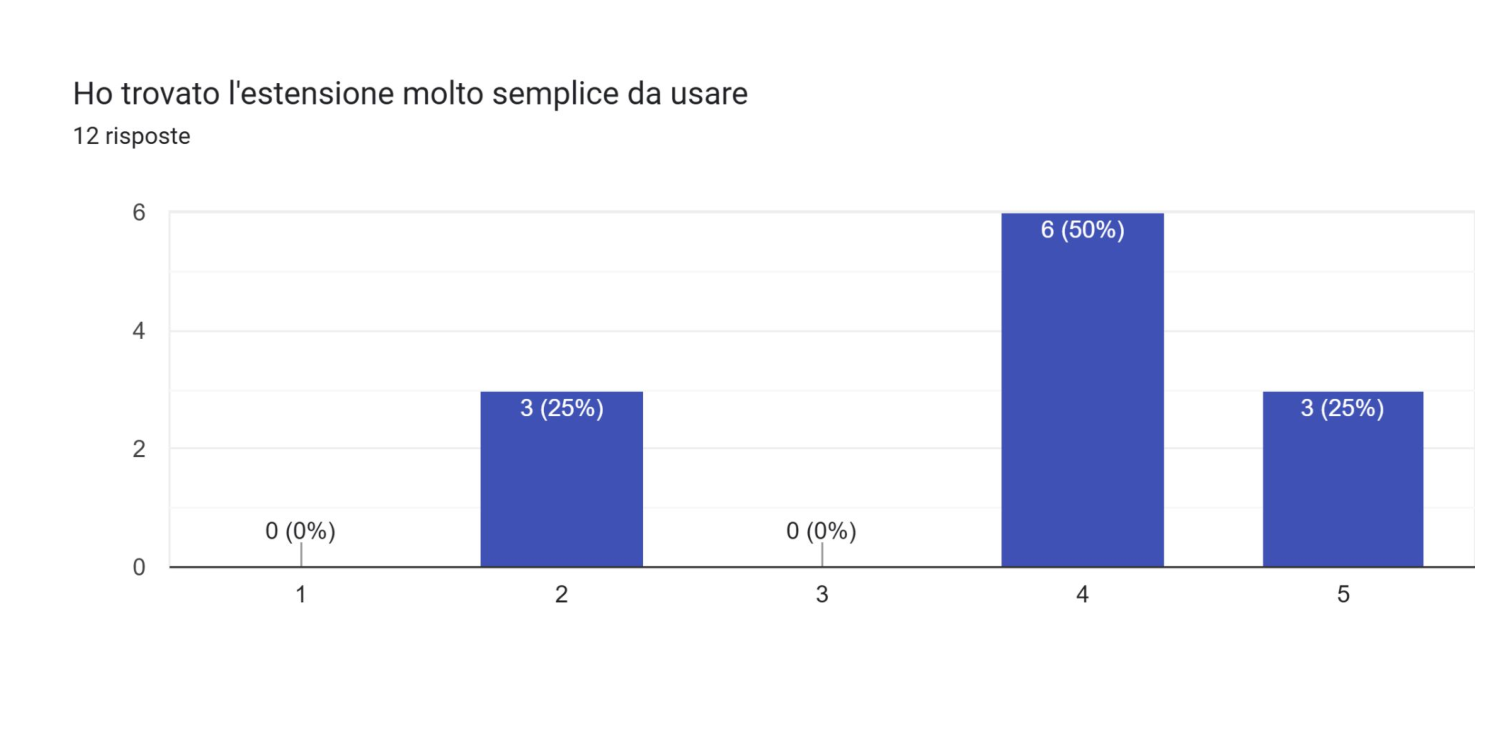
\includegraphics[width=0.95\columnwidth]{sus/domanda_3.pdf}
    \caption{Risposte alla domanda 3}
    \label{fig:sus_q3}
  \end{figure}
\end{minipage}

\subsubsection*{Domanda 4}

\vspace{5pt}
\begin{minipage}{\textwidth}
  \par\noindent La figura \ref{fig:sus_q4} mostra le risposte alla quarta domanda del questionario \gls{sus}.
  \begin{figure}[H]
    \centering
    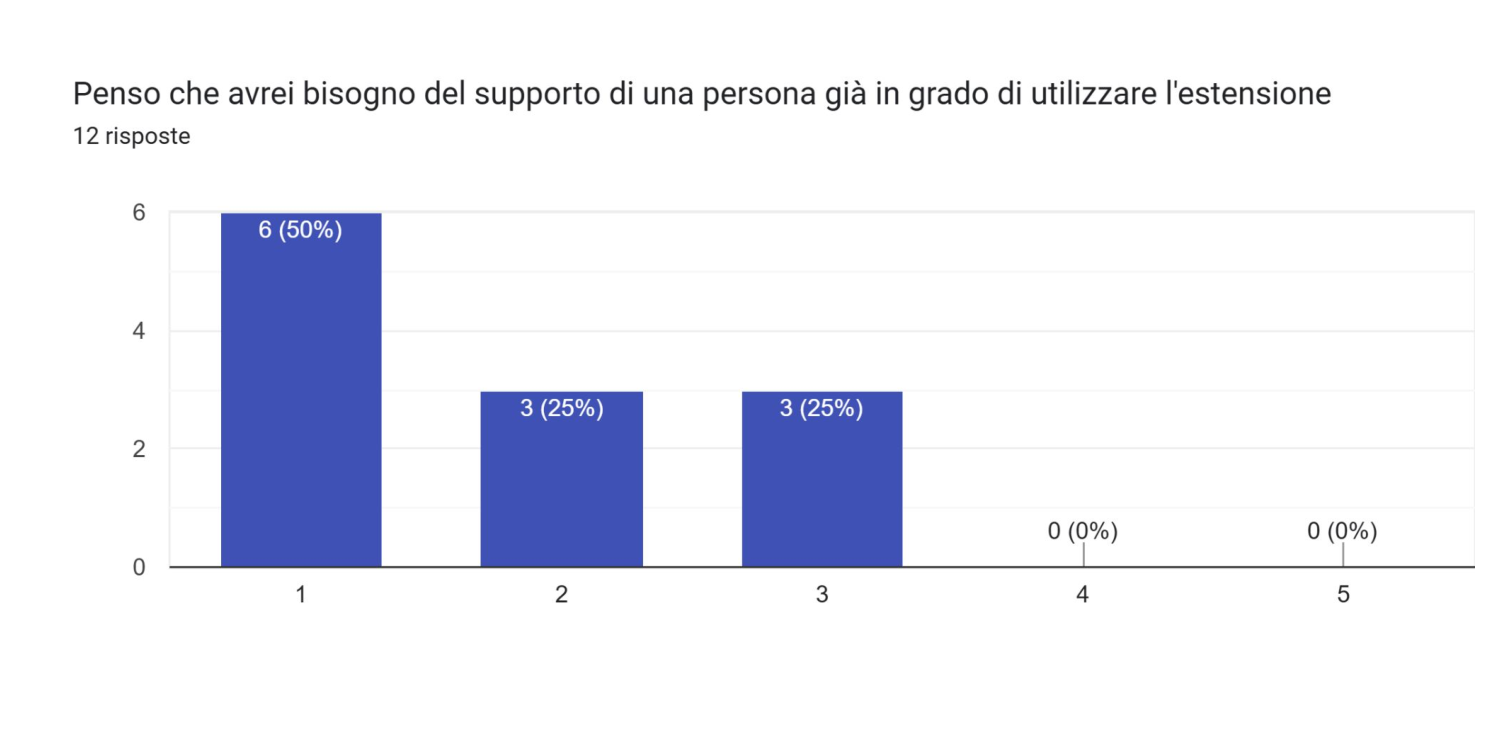
\includegraphics[width=0.95\columnwidth]{sus/domanda_4.pdf}
    \caption{Risposte alla domanda 4}
    \label{fig:sus_q4}
  \end{figure}
\end{minipage}

\subsubsection*{Domanda 5}

\vspace{5pt}
\begin{minipage}{\textwidth}
  \par\noindent La figura \ref{fig:sus_q5} mostra le risposte alla quinta domanda del questionario \gls{sus}.
  \begin{figure}[H]
    \centering
    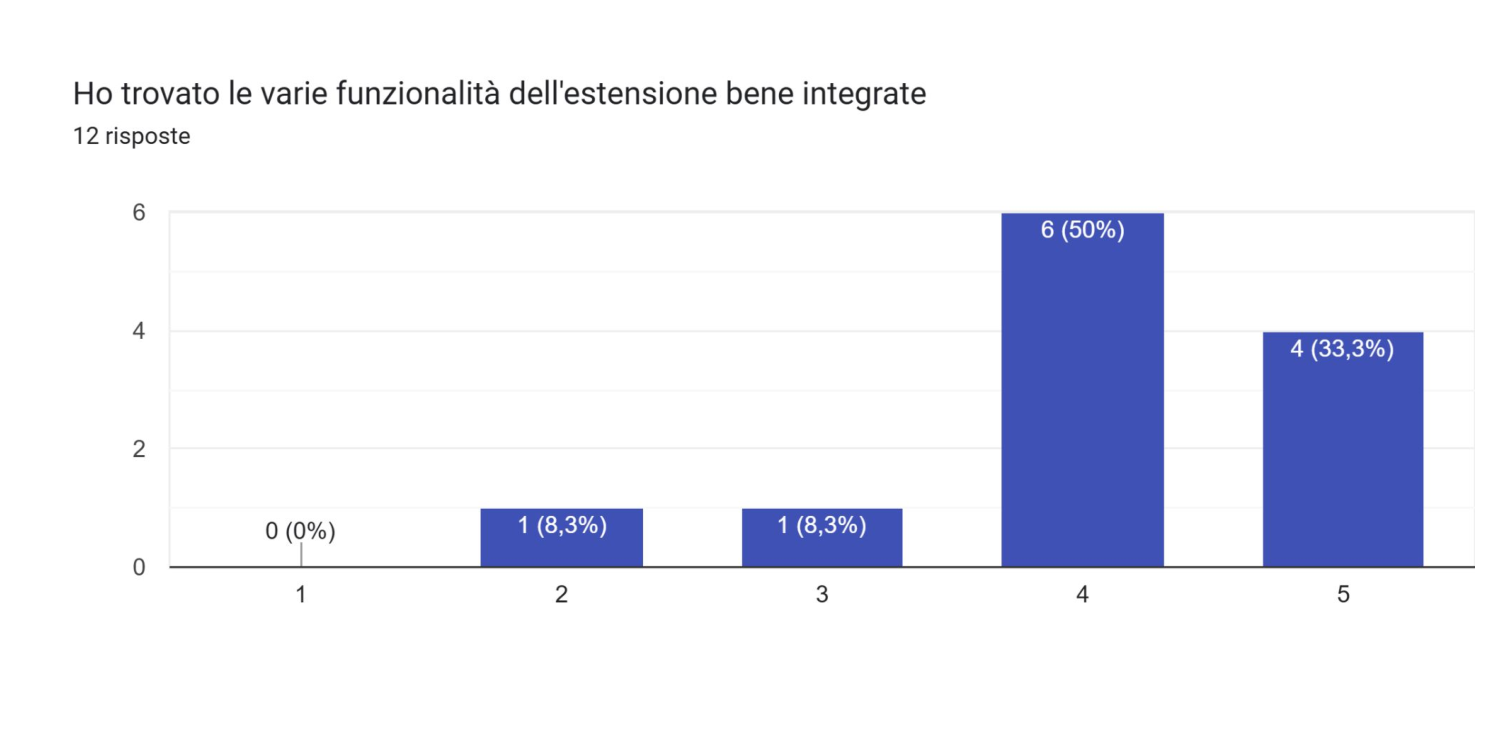
\includegraphics[width=0.95\columnwidth]{sus/domanda_5.pdf}
    \caption{Risposte alla domanda 5}
    \label{fig:sus_q5}
  \end{figure}
\end{minipage}

\subsubsection*{Domanda 6}

\vspace{5pt}
\begin{minipage}{\textwidth}
  \par\noindent La figura \ref{fig:sus_q6} mostra le risposte alla sesta domanda del questionario \gls{sus}.
  \begin{figure}[H]
    \centering
    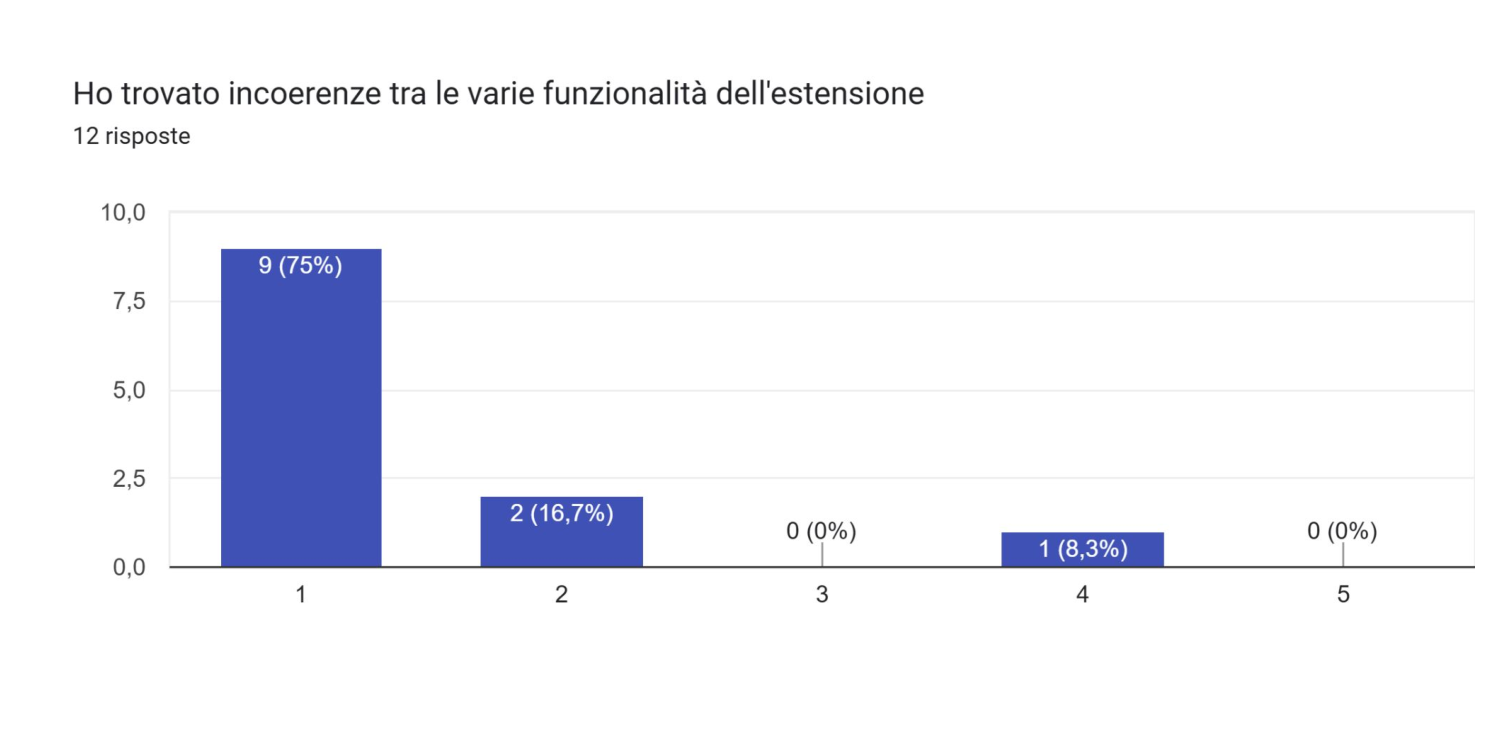
\includegraphics[width=0.95\columnwidth]{sus/domanda_6.pdf}
    \caption{Risposte alla domanda 6}
    \label{fig:sus_q6}
  \end{figure}
\end{minipage}

\subsubsection*{Domanda 7}

\vspace{5pt}
\begin{minipage}{\textwidth}
  \par\noindent La figura \ref{fig:sus_q7} mostra le risposte alla settima domanda del questionario \gls{sus}.
  \begin{figure}[H]
    \centering
    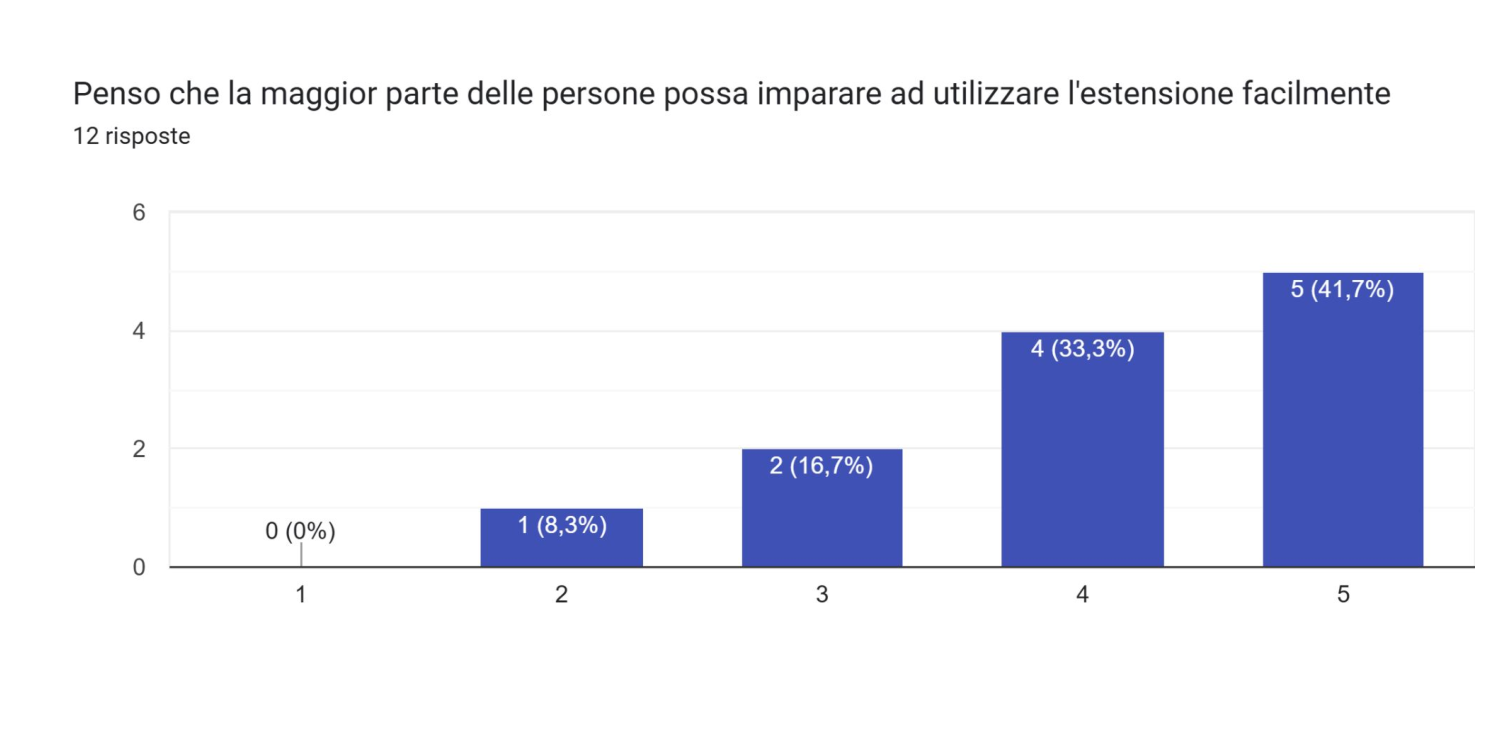
\includegraphics[width=0.95\columnwidth]{sus/domanda_7.pdf}
    \caption{Risposte alla domanda 7}
    \label{fig:sus_q7}
  \end{figure}
\end{minipage}

\subsubsection*{Domanda 8}

\vspace{5pt}
\begin{minipage}{\textwidth}
  \par\noindent La figura \ref{fig:sus_q8} mostra le risposte all'ottava domanda del questionario \gls{sus}.
  \begin{figure}[H]
    \centering
    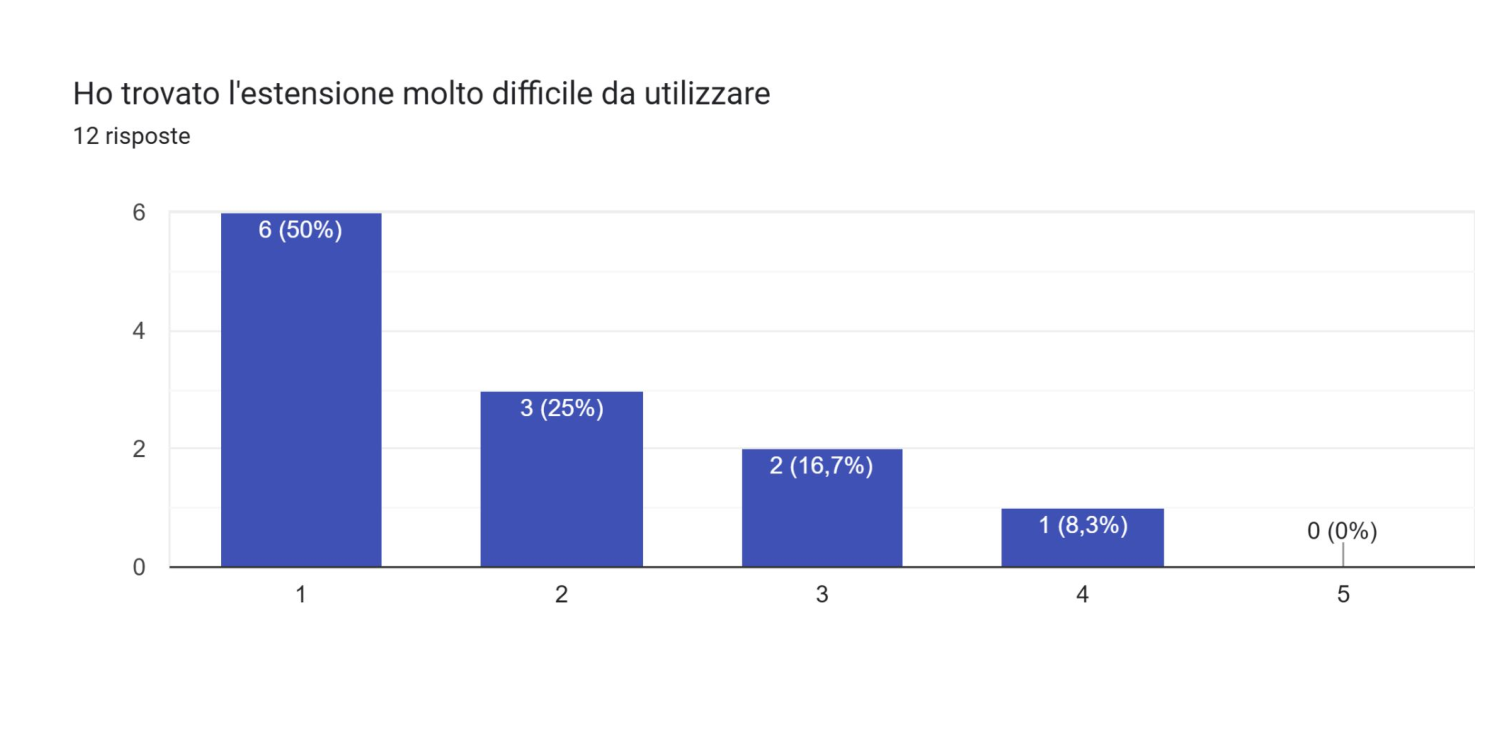
\includegraphics[width=0.95\columnwidth]{sus/domanda_8.pdf}
    \caption{Risposte alla domanda 8}
    \label{fig:sus_q8}
  \end{figure}
\end{minipage}

\subsubsection*{Domanda 9}

\vspace{5pt}
\begin{minipage}{\textwidth}
  \par\noindent La figura \ref{fig:sus_q9} mostra le risposte alla nona domanda del questionario \gls{sus}.
  \begin{figure}[H]
    \centering
    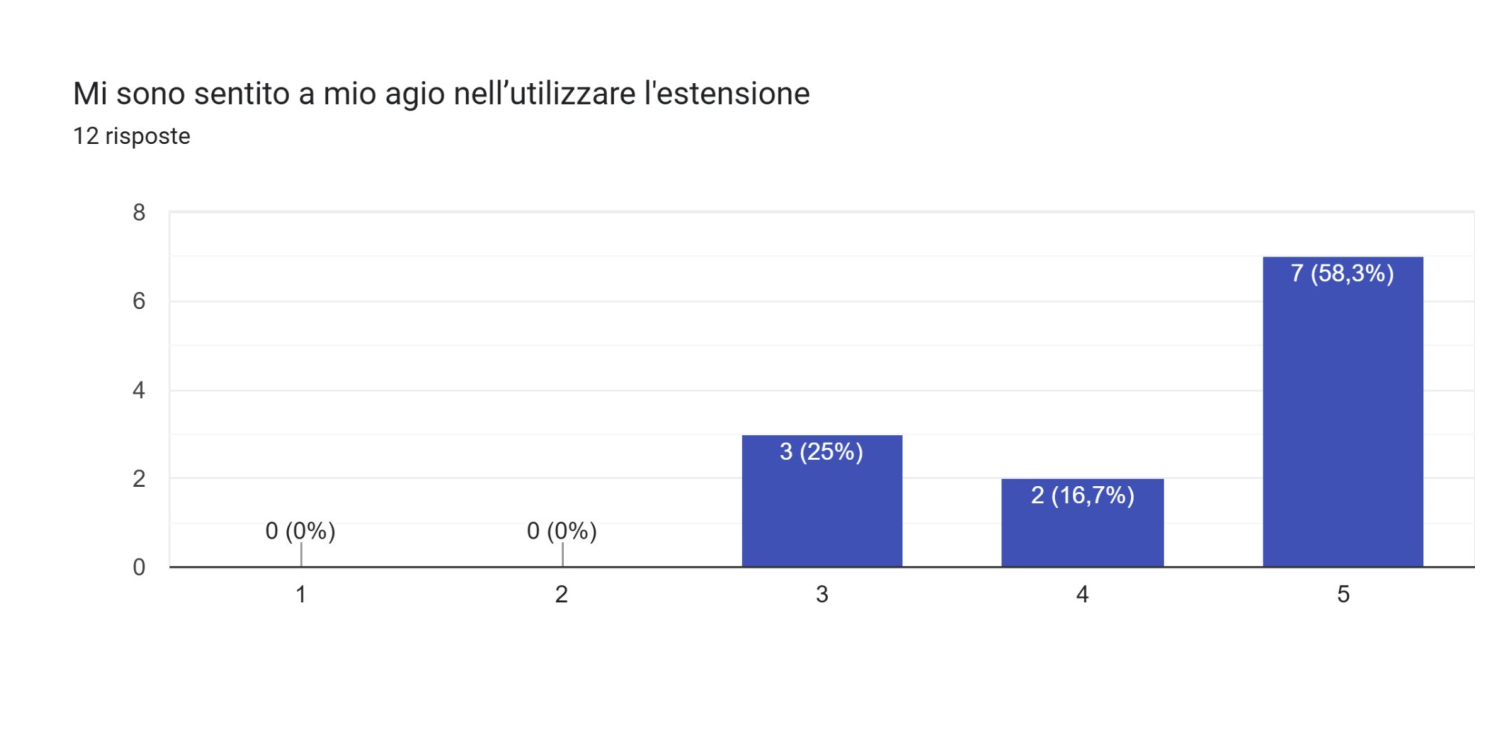
\includegraphics[width=0.95\columnwidth]{sus/domanda_9.pdf}
    \caption{Risposte alla domanda 9}
    \label{fig:sus_q9}
  \end{figure}
\end{minipage}

\subsubsection*{Domanda 10}

\vspace{5pt}
\begin{minipage}{\textwidth}
  \par\noindent La figura \ref{fig:sus_q10} mostra le risposte alla decima domanda del questionario \gls{sus}.
  \begin{figure}[H]
    \centering
    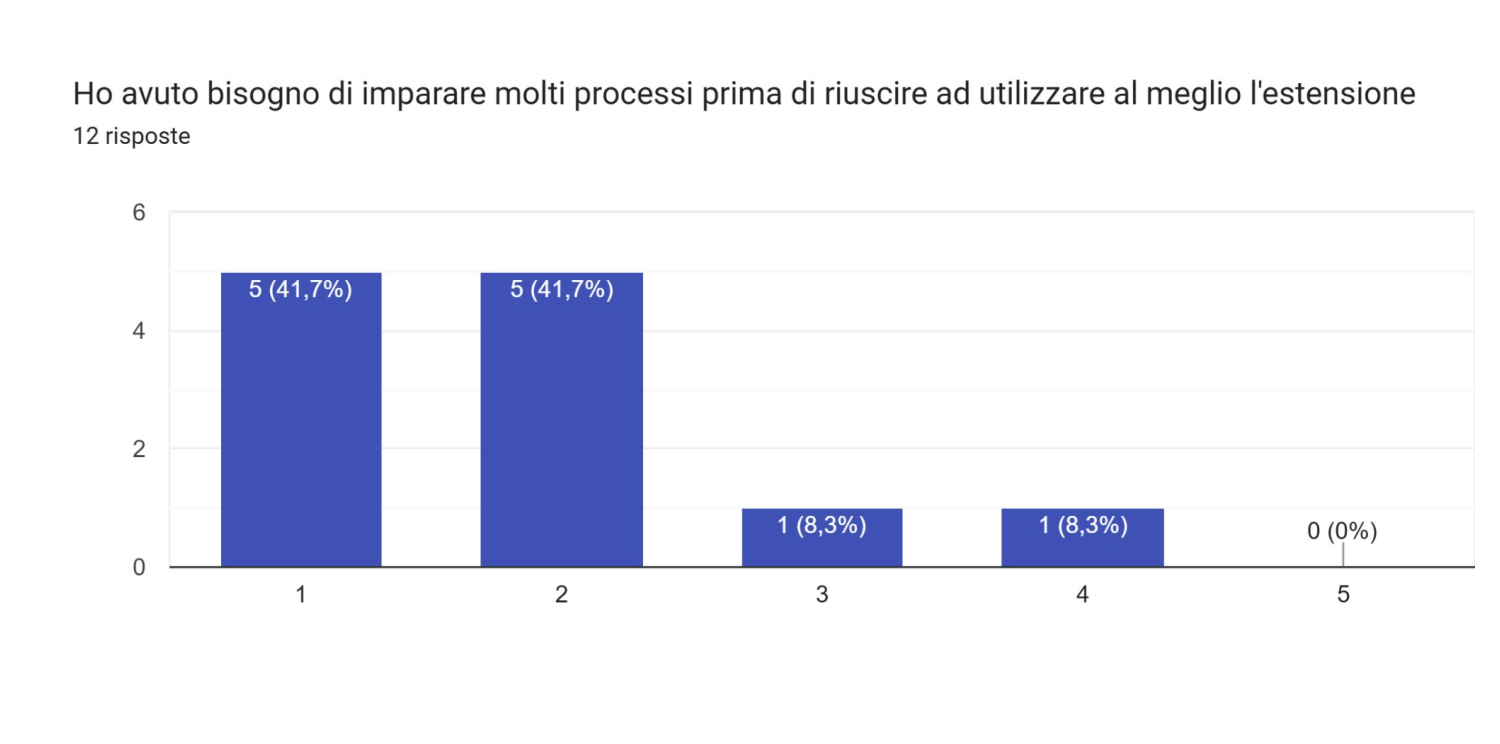
\includegraphics[width=0.95\columnwidth]{sus/domanda_10.pdf}
    \caption{Risposte alla domanda 10}
    \label{fig:sus_q10}
  \end{figure}
\end{minipage}

\newpage

\section{Accessibilità}

\par Dal momento che lo strumento di analisi delle parole chiave è integrato in un’estensione preesistente orientata all’accessibilità, anche questo \textit{tool} è stato progettato in conformità alle linee guida \gls{wcag}. A tal fine, sono stati condotti test di accessibilità con i seguenti obiettivi:
\begin{itemize}
  \item Verificare il rispetto del \textbf{rapporto minimo di contrasto} tra testo e sfondo, pari a 4.5:1 per il testo di dimensioni “normali” e 3:1 per il testo di grandi dimensioni. Questo controllo è stato applicato sia agli elementi interni all’estensione, sia a quelli utilizzati per evidenziare le parole chiave;
  \item Controllare che le \textbf{immagini non decorative} siano dotate di un testo alternativo;
  \item Accertarsi che le \textbf{icone non decorative} siano accompagnate da un’etichetta accessibile;
  \item Verificare l’accessibilità dei \textbf{tooltip}, assicurandosi che vengano attivati e disattivati correttamente quando si interagisce con l’elemento \textit{trigger}, sia tramite navigazione da tastiera sia tramite l’uso del mouse. Inoltre, i tooltip devono rimanere visibili al passaggio del mouse su di essi e devono poter essere chiusi premendo il tasto Esc;
  \item Controllare che tutti gli \textbf{elementi interattivi} (come pulsanti o link) dispongano di un’etichetta testuale descrittiva;
  \item Assicurare la \textbf{navigazione tramite tastiera}, con un ordine di tabulazione logico e una chiara indicazione visiva dell’elemento attualmente attivo.
\end{itemize}

\vspace{15pt}
\par\noindent Tutti i test eseguiti, sia manuali che automatici (condotti principalmente con \textit{axe DevTools} e \textit{Colour Contrast Analyser}), hanno dato esito positivo.
